\documentclass[serif]{beamer}
%\usepackage[utopia]{mathdesign}
%\usepackage[no-math]{fontspec}
%\setmainfont{Liberation Serif}

\usepackage{minted}
\usepackage{hyperref}
\usepackage{ccicons}

%gets rid of bottom navigation bars
\setbeamertemplate{footline}[page number]{}

%gets rid of navigation symbols
\setbeamertemplate{navigation symbols}{}

\title[Systemd security features]{Securing your daemons using systemd}
\author{Zbigniew Jędrzejewski-Szmek}
\institute{%
  \includegraphics{beamer-themeredhat/redhat.png}\\
  \medskip
  \textit{zbyszek@in.waw.pl}\\
  \medskip
  \ccbysa
}
\date{\tiny FOSDEM, Brussels, 2020.2.2}

\begin{document}
\begin{frame}
\titlepage % Print the title page as the first slide
\end{frame}

\begin{frame}
  \frametitle{About me}

  systemd upstream\\
  Fedora (FESCo, systemd maint., Python SIG, Rust SIG)

\end{frame}

\begin{frame}[fragile]
  \frametitle{Before we begin...\\Why use systemd for this at all?}

  \begin{itemize}
  \item centralization
  \item abstraction of hardware architecture / kernel version
  \item unprivileged operation
  \end{itemize}

  \pause
  \bigskip

  Numbers:
  \begin{minted}{bash}
$ dnf repoquery --releasever=32 -l --whatprovides \
    '/usr/lib/systemd/system/*' \
    rg -i '^/usr/lib/systemd/system/[a-z0-9_@.\\-]+$' | \
    sort -u | wc -l
1740!!!
  \end{minted}

\end{frame}

\begin{frame}[fragile]
  \frametitle{Before we begin...\\Unit files}

  \pause

  \begin{minted}{ini}
    # /etc/systemd/system/mydaemon.service
    [Service]
    ExecStart=/usr/local/bin/mydaemon
  \end{minted}
  \begin{minted}{console}
    $ sudo systemctl start mydaemon.service
  \end{minted}

  \medskip
  \pause

  \begin{minted}{console}
    $ sudo /usr/local/bin/mydameon
  \end{minted}

  \medskip
  \pause

  \begin{minted}{console}
    $ sudo systemd-run /usr/local/bin/mydameon
    $ sudo systemd-run -t /usr/local/bin/mydameon
  \end{minted}
\end{frame}

\begin{frame}[fragile]
  \frametitle{Basics}
  \pause
  \texttt{User=}

  \medskip
  \pause

  \begin{minted}{console}
    $ systemd-run whoami
    root

    $ systemd-run --uid=zbyszek whoami
    zbyszek
    $ systemd-run -p User=zbyszek whoami
    zbyszek
  \end{minted}
\end{frame}

\begin{frame}
  \frametitle{Limiting access to the file system}
  \begin{itemize}
  \item \texttt{ProtectHome=yes|read-only}
  \item \texttt{ProtectSystem=yes|full|strict}
    \pause

  \item \texttt{InaccessiblePaths=}
  \item \texttt{ReadOnlyPaths=}
  \item \texttt{ReadWritePaths=}

    \pause
  \item \texttt{\textcolor{gray}{BindPaths=}}
  \item \texttt{\textcolor{gray}{ReadOnlyBindPaths=}}

  \end{itemize}
\end{frame}

\begin{frame}
  \frametitle{Limiting access to the file system}

  \begin{itemize}
  \item \texttt{PrivateTmp=yes}
  \end{itemize}
\end{frame}

\begin{frame}
  \frametitle{Limiting access to the file system\\a better way}
  \pause
  \begin{columns}
    \begin{column}{0.6\textwidth}
      \begin{itemize}
      \item \texttt{RuntimeDirectory=\textit{foo}}
      \item \texttt{StateDirectory=\textit{foo}}
      \item \texttt{CacheDirectory=\textit{foo}}
      \item \texttt{LogsDirectory=\textit{foo}}
      \item \texttt{ConfigurationDirectory=\textit{foo}}
      \end{itemize}
    \end{column}
    \color{gray}
    \begin{column}{0.4\textwidth}
      /run/\textit{foo}/ \\[.32em]
      /var/lib/\textit{foo}/ \\[.32em]
      /var/cache/\textit{foo}/ \\[.32em]
      /var/log/\textit{foo}/ \\[.32em]
      /etc/\textit{foo}/
    \end{column}
  \end{columns}
\end{frame}

\begin{frame}[fragile]
  \begin{minted}{console}
$ sudo systemd-run -t -p User=zbyszek \
                      -p RuntimeDirectory=foo \
                      ls -ld /run/foo
  \end{minted}

  \begin{itemize}
  \item automatic \textit{creation} and \textit{ownership}
  \item automatic \textit{removal}
  \end{itemize}
\end{frame}

\begin{frame}[fragile]
  \frametitle{User creation on demand?}
  \pause
  \begin{itemize}
  \item \texttt{DynamicUser=yes}
  \end{itemize}

  \pause

  \begin{minted}{console}
$ systemd-run -p DynamicUser=1 -t whoami
  \end{minted}
\pause
  \begin{minted}{console}
run-u215640
\end{minted}
  \pause

  \begin{minted}{console}
$ echo -e 'asdf\nasdf' | \
  \end{minted}
  \pause
  \begin{minted}{bash}
  systemd-run --pipe -p DynamicUser=1 \
    bash -c 'grep .; whoami' | \
  \end{minted}
  \pause
  \begin{minted}{bash}
  systemd-run --pipe -p DynamicUser=1 \
    bash -c 'grep .; whoami' | \
  \end{minted}
  \pause
  \begin{minted}{bash}
  systemd-run --pipe -p DynamicUser=1 \
    bash -c 'grep .; whoami'
  \end{minted}
\end{frame}

\begin{frame}
  \frametitle{What about the network?}

  \pause

  \begin{itemize}
  \item \texttt{PrivateNetwork=yes}
  \end{itemize}

  \pause

  ``\texttt{PrivateNetwork=yes} is the recommeded way to run network services''
\end{frame}

\begin{frame}[c]
  \frametitle{Socket Activation}

  A daemon does not open a socket itself, it receives a socket from the manager

  \medskip
  \pause

  \centering
  Two types of socket activation:

  \medskip

  \begin{columns}
    \begin{column}{0.5\textwidth}
      \texttt{Accept=yes}\\
      → a single instance of the service is started for each connection\\
      → ``wait'' under inetd/xinetd
    \end{column}
    \begin{column}{0.5\textwidth}
      \texttt{Accept=no}\\
      → a single instance of the service is started for each connection\\
      → ``nowait'' under inetd/xinetd
    \end{column}
  \end{columns}
\end{frame}

\begin{frame}
  \frametitle{Per-service network firewall}

  \begin{itemize}
  \item \texttt{IPAddressAllow=\color{gray}10.20.30.0/24 1.2.3.4}
  \item \texttt{IPAddressDeny=\color{gray}*}
  \item \texttt{IP\{Ingress,Egress\}FilterPath=}
  \end{itemize}

  BPF!
\end{frame}

\begin{frame}[c]
  \Huge{Low-level stuff}
\end{frame}

\begin{frame}
  \begin{itemize}
  \item \texttt{MemoryDenyWriteExecute=yes}
  \item \texttt{PrivateDevices=yes}
  \item \texttt{NoNewPrivileges=yes}
  \item \texttt{RestrictSUIDSGID=yes}
  \item \texttt{ProtectKernelTunables=yes}
  \item \texttt{ProtectClock=yes}
  \item \texttt{ProtectHostname=yes}
  \item \texttt{ProtectKernelLogs=yes}
  \item \texttt{LockPersonality=yes}
  \end{itemize}
\end{frame}

\begin{frame}
  \frametitle{Capability limits}

  \begin{itemize}
  \item \texttt{CapabilityBoundingSet=}
  \item \texttt{\textcolor{gray}{Capability=}}
  \item \texttt{\textcolor{gray}{DropCapability=}}
  \item \texttt{AmbientCapabilities=}
  \end{itemize}
\end{frame}

\begin{frame}[fragile]
  \frametitle{System call filtering}
  \framesubtitle{``seccomp mode 2''}

  \pause

  \begin{itemize}
  \item \texttt{SyscallFilter=...}\\
        implemented using \texttt{libseccomp}
  \item \texttt{syscall1 | syscall2 | @group}
  \item \texttt{@basic-io}
  \item \texttt{\~@obsolete}

  \medskip
  \pause

  \item \texttt{SystemCallArchitectures=native\color{gray}|x86\_64|i386|...}
  \item \texttt{RestrictAddressFamilies=AF\_UNIX|AF\_INET|AF\_INET6
        \color{gray}|AF\_CAN|AF\_APPLETALK|...}

  \end{itemize}

  \medskip
  \pause

  \begin{minted}{console}
$ systemd-analyze syscall-filter @obsolete
  \end{minted}
\end{frame}

\begin{frame}[fragile]
  \frametitle{\texttt{systemd-analyze security}}

  \begin{minted}{console}
$ systemd-analyze security systemd-resolved.service
  \end{minted}
\end{frame}

\begin{frame}
  \frametitle{Fedora 32: \texttt{systemd-analyze security *}}

  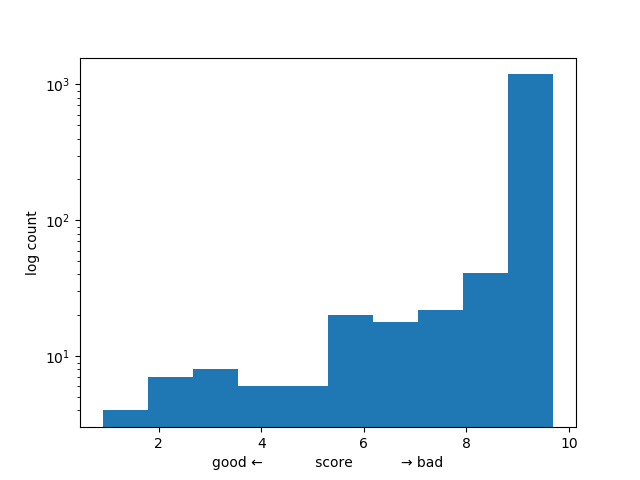
\includegraphics[width=\textwidth]{images/fedora-scores.png}
\end{frame}

\begin{frame}
  \frametitle{Stacking}

  the application\\
  systemd sandboxing\\
  selinux | apparmor | ...\\
  kernel
\end{frame}


\begin{frame}[fragile]
  \textcolor{gray}{The End}

  \bigskip

  \url{https://github.com/systemd/systemd}\\
  docs: \url{https://systemd.io/}\\
  \phantom{docs: }\url{https://www.freedesktop.org/wiki/Software/systemd/}\hspace*{-5cm}\\

  \medskip
  this:\\
  \url{https://github.com/keszybz/systemd-security-talk/blob/master/systemd-security.pdf}
\end{frame}

\end{document}
